\documentclass[10pt]{article}

\usepackage{spheric}
%%%TITLE
\title{Application of Improved SPH Solid-Wall Boundary Model in Missile Waterexiting}
\date{}

%%AFFILIATIONS
\author[$\relax$]{Zheng Hua-lin}
\author[$\relax$]{Qiang Hong-fu}
\author[$\relax$]{Chen Fu-zhen}
\author[$\relax$]{Shi Chao}
\affil[$\relax$]{Department of Power Engineering, Xi'an Hi-Tech Institute, China}
\affil[$\relax$]{\email{}{zero2one@aliyun.com}}


%%DOCUMENT
\begin{document}

\maketitle

%\SelectedTopics{}

%%PLEASE PUT YOUR ABSTRACT HERE
\begin{abstract}
For its meshfree nature, smoothed particle hydrodynamics (SPH) faces challenges on solving rigid-fluid interaction problems. By correcting the condition and force direction between fluid particles and boundary particles, an improved SPH solid-wall boundary model is proposed by Liu \cite{hu2015new}, which can apply boundary condition effectively. The classical dambreak problem are simulated, which are respectively compared with the experimental results and another simulation results.

And with this treatment, the 2-D missile waterexiting problem is simulated, which explores the influence of water depth and velocity at the ignition point on the process of missile waterexiting. The present study expands application of SPH method in solving rigid-fluid interaction problems, and with the help of it, the stable flow field, smooth velocity and pressure fields could be obtained.

\begin{figure}[!htb]
\centering
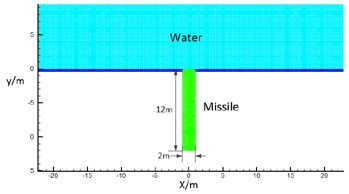
\includegraphics[width=0.46\textwidth]{36-11.png}~~
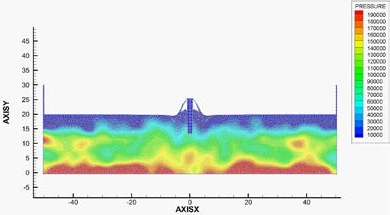
\includegraphics[width=0.46\textwidth]{36-12.png}
\caption{model of missile waterexiting (left) and schematic diagram of the process of missile waterexiting (right).}\label{fig:36}
\end{figure}

\end{abstract}


%%THE END OF ABSTRACT

\addbib

\end{document}
